%! TEX program = lualatex
\pdfvariable minorversion=7
\documentclass[10pt]{article}

% Packages
\usepackage[no-math]{fontspec}
\usepackage{geometry}
\usepackage{hyperref}
\usepackage[backend=biber]{biblatex} % we use the biber implementation of biblatex for bibliographies
\usepackage[nonumberlist, toc]{glossaries}
\usepackage{graphicx}
\usepackage{pdfpages}
\usepackage{booktabs}
\usepackage{float}
\usepackage{subcaption}
\usepackage{fancyhdr}
\usepackage{amsmath}
\usepackage{siunitx}

% Formatting
\geometry{letterpaper, portrait, margin=.85in}
\defaultfontfeatures{Ligatures=TeX}
\setmainfont[
    BoldFont       = Avenir Medium,
    ItalicFont     = Avenir Book Oblique,
    BoldItalicFont = Avenir Medium Oblique
]{Avenir Book}
\setmonofont{Andale Mono}
\sisetup{detect-all} % used by siunitx to always typeset units in the font of the current environment
\urlstyle{same}

\newcommand\theteamname{Midnight Sun Solar Car Team} % should not change normally
\newcommand\theuniversityname{University of Waterloo} % should also not change normally
\newcommand\theteamwebsite{www.uwmidsun.com} % should also not normally change
\newcommand\theteamphone{(519) 888-4567 x32978} % should also not normally change

\newcommand\thetitle{Solar Cell Tech Report} % <--------------- add the title
\newcommand\thesubtitle{Electrical} % <--------------- add a subtitle or leave the field empty
\newcommand\theauthor{Minghao Ji} % <--------------- add an author with contact info or comment this line
\newcommand\theauthorcontact{minghao.ji@uwmidsun.com} % <--------------- add author's email or leave the field empty
\newcommand\thedate{\today} % <--------------- update the date, use this format

\pagestyle{fancy}
\renewcommand{\headrulewidth}{0pt}
\lhead{\thetitle}
\rhead{\theteamname}

\begin{document}

% Title Page
\begin{titlepage}
\large
\vspace*{2cm}
\centering

\includegraphics[width=.25\textwidth]{./figures/midnightSunLogoCircle.png} \\
\vspace{1.5cm}
{\LARGE \theteamname} \\
\theuniversityname \\
\vspace{2.2cm}
{\LARGE MSXII} \\
\vspace{0.4cm}
{\huge\bfseries \thetitle} \\
\vspace{0.2cm}
{\LARGE \thesubtitle} \\
\vspace{2.2cm}
\ifdefined \theauthor
\par Prepared by: \\
\theauthor \\
\theauthorcontact \\
\fi
\thedate \\
\vfill
\theteamwebsite \\
\theteamphone
\end{titlepage}

% Main Matter
\tableofcontents
\listoffigures % <-------------- uncomment for list of figures
%\listoftables % <-------------- uncomment for list of tables

\section{Manufacturer}
% Manufacturer’s name and contact information
% Stock number, type, or description
MSXII uses SunPower Gen E (E60), bin Le1 cells. They are manufactured by SunPower Corporation. The team's primary point of contact for cell ordering was Scott McHugo. His email and phone number on record is scott.mchugo@sunpower.com and +1 (408) 240-5500.

Scott is the regional representative for SunPower in the Americas but helped the team organize purchasing and shipping of cells from SunPower's european operations to an array manufacturer in Germany.

\section{Specifications}
% Manufacturer’s quote for cell area (cm2)
SunPower's quote for the Gen E bin Le1 cell area is \SI{153.328}{\centi\metre\squared}.
% Manufacturer’s quote for performance
Their quote for cell performance is \SI{23.7}{\percent} efficiency, yielding a typical power output of \SI{3.63}{\watt} per cell.
% Cost (USD) per cell
The cost per cell quoted to the team, excluding shipping and handling, is EUR 5.21. The equivalent cost in USD quoted by SunPower is USD 6.38.

\section{Layout}
MSXII has a total of 322 full-cells and 8 half-cells, yielding a total cell area below the equivalent of 326 full-cells. Based on SunPower's quoted cell area of \SI{153.328}{\centi\metre\squared}, this gives a total absolute area under \SI{49985}{\centi\metre\squared}, meeting ASC regulations. A CAD drawing of the cell layout and MPPT layout is shown in Figure \ref{fig:array-layout}.

\begin{figure}[hbp]
\centering
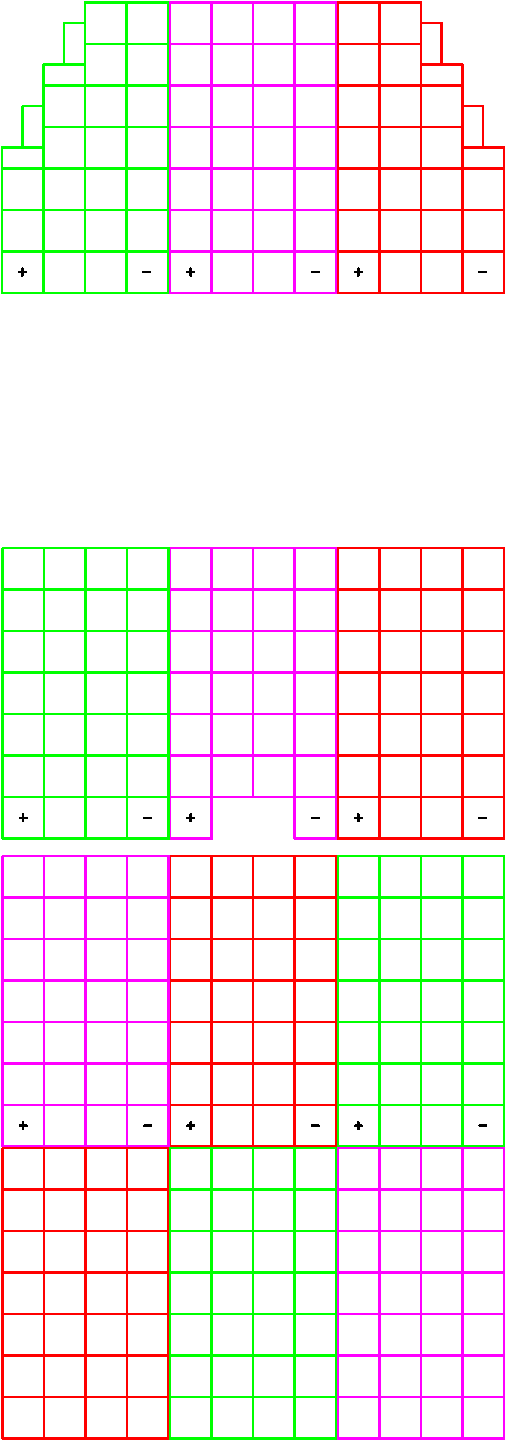
\includegraphics[width=0.45\textwidth]{figures/array-cell-layout}
\hfill
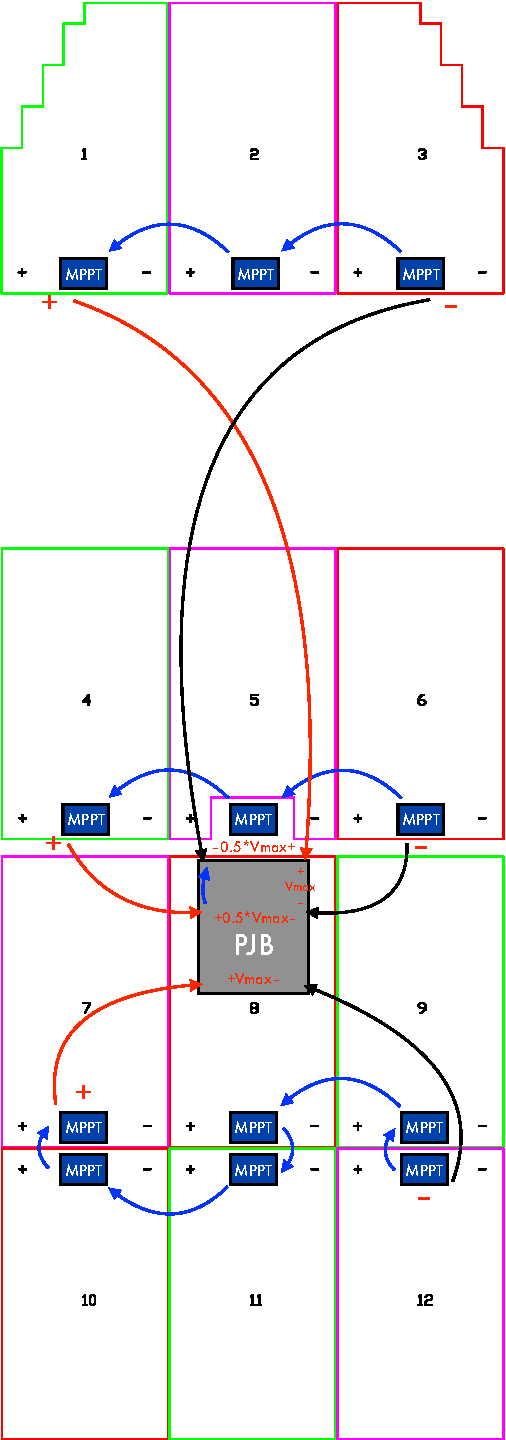
\includegraphics[width=0.45\textwidth]{figures/array-mppt-layout}
\caption{Cell and MPPT layout}
\label{fig:array-layout}
\end{figure}

\clearpage

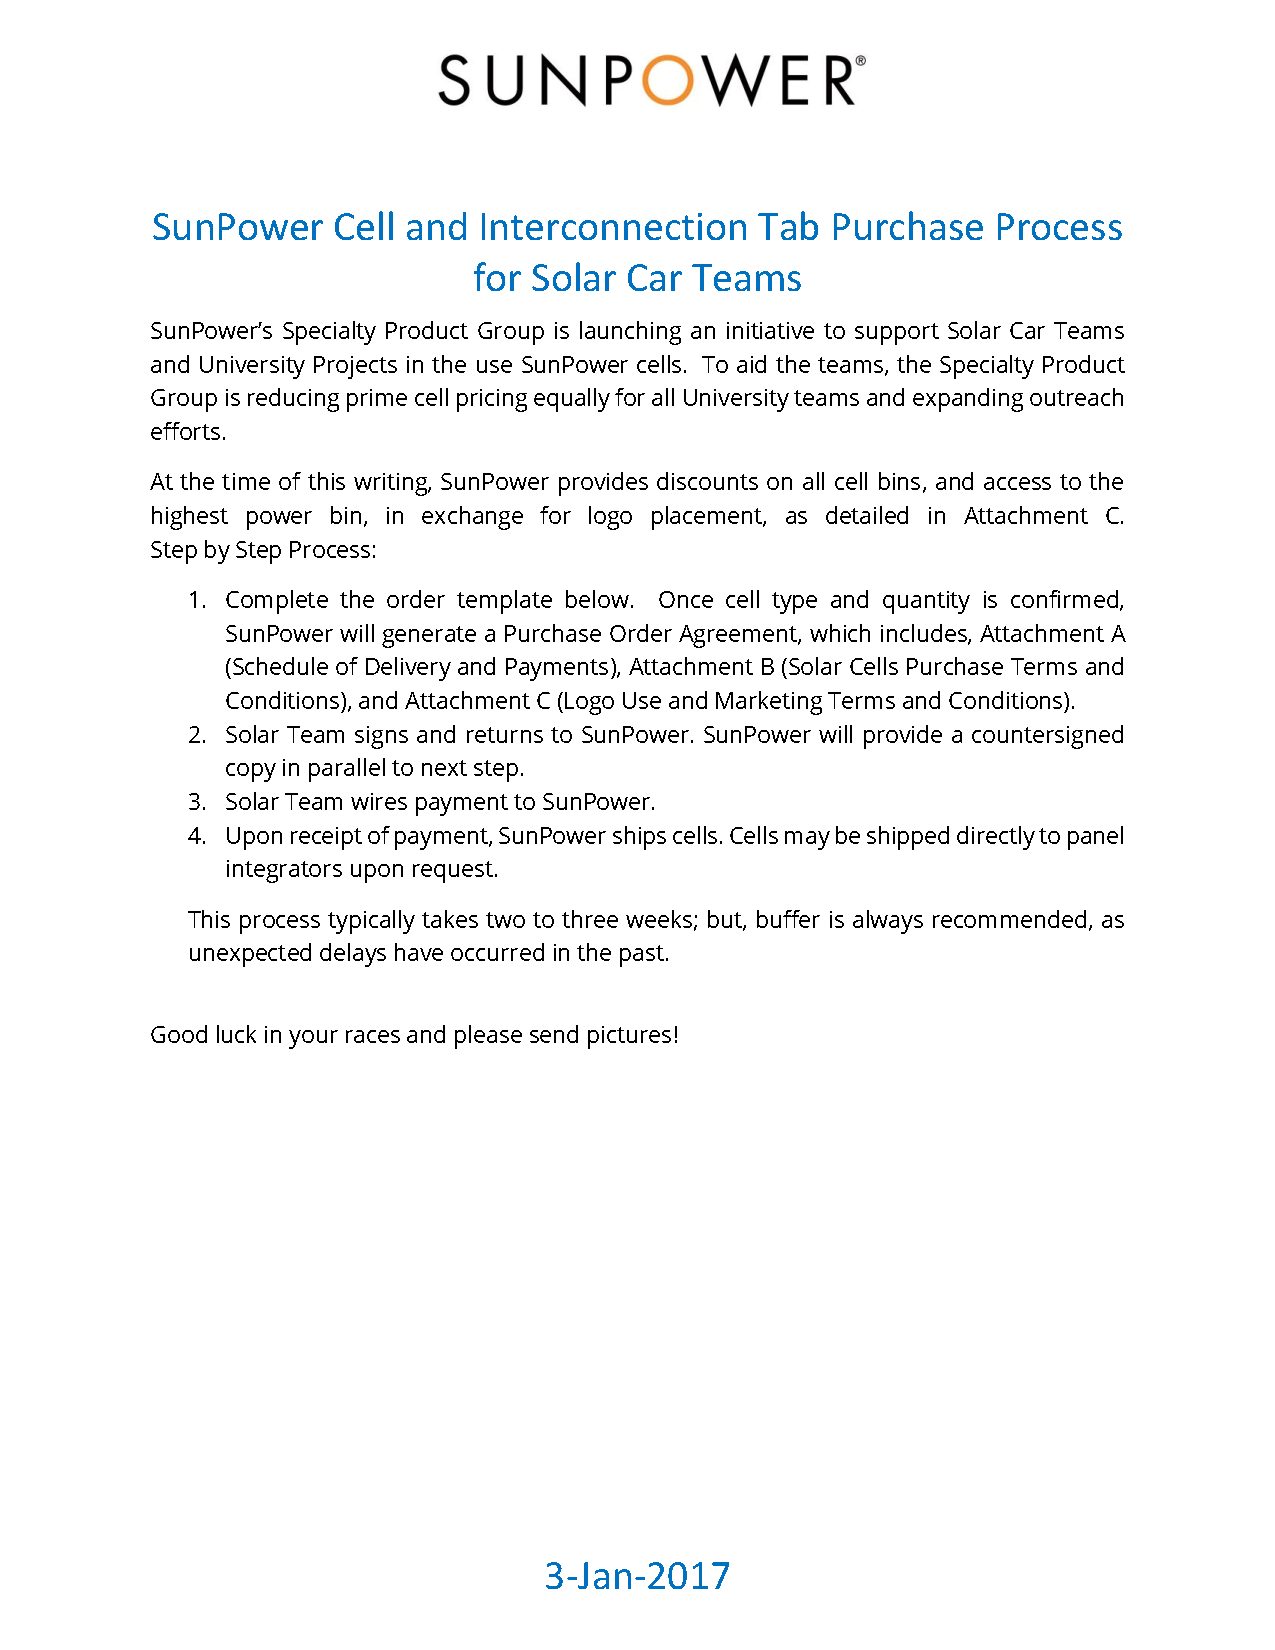
\includepdf[pages={-}]{pages/sunpower-university-teams.pdf}
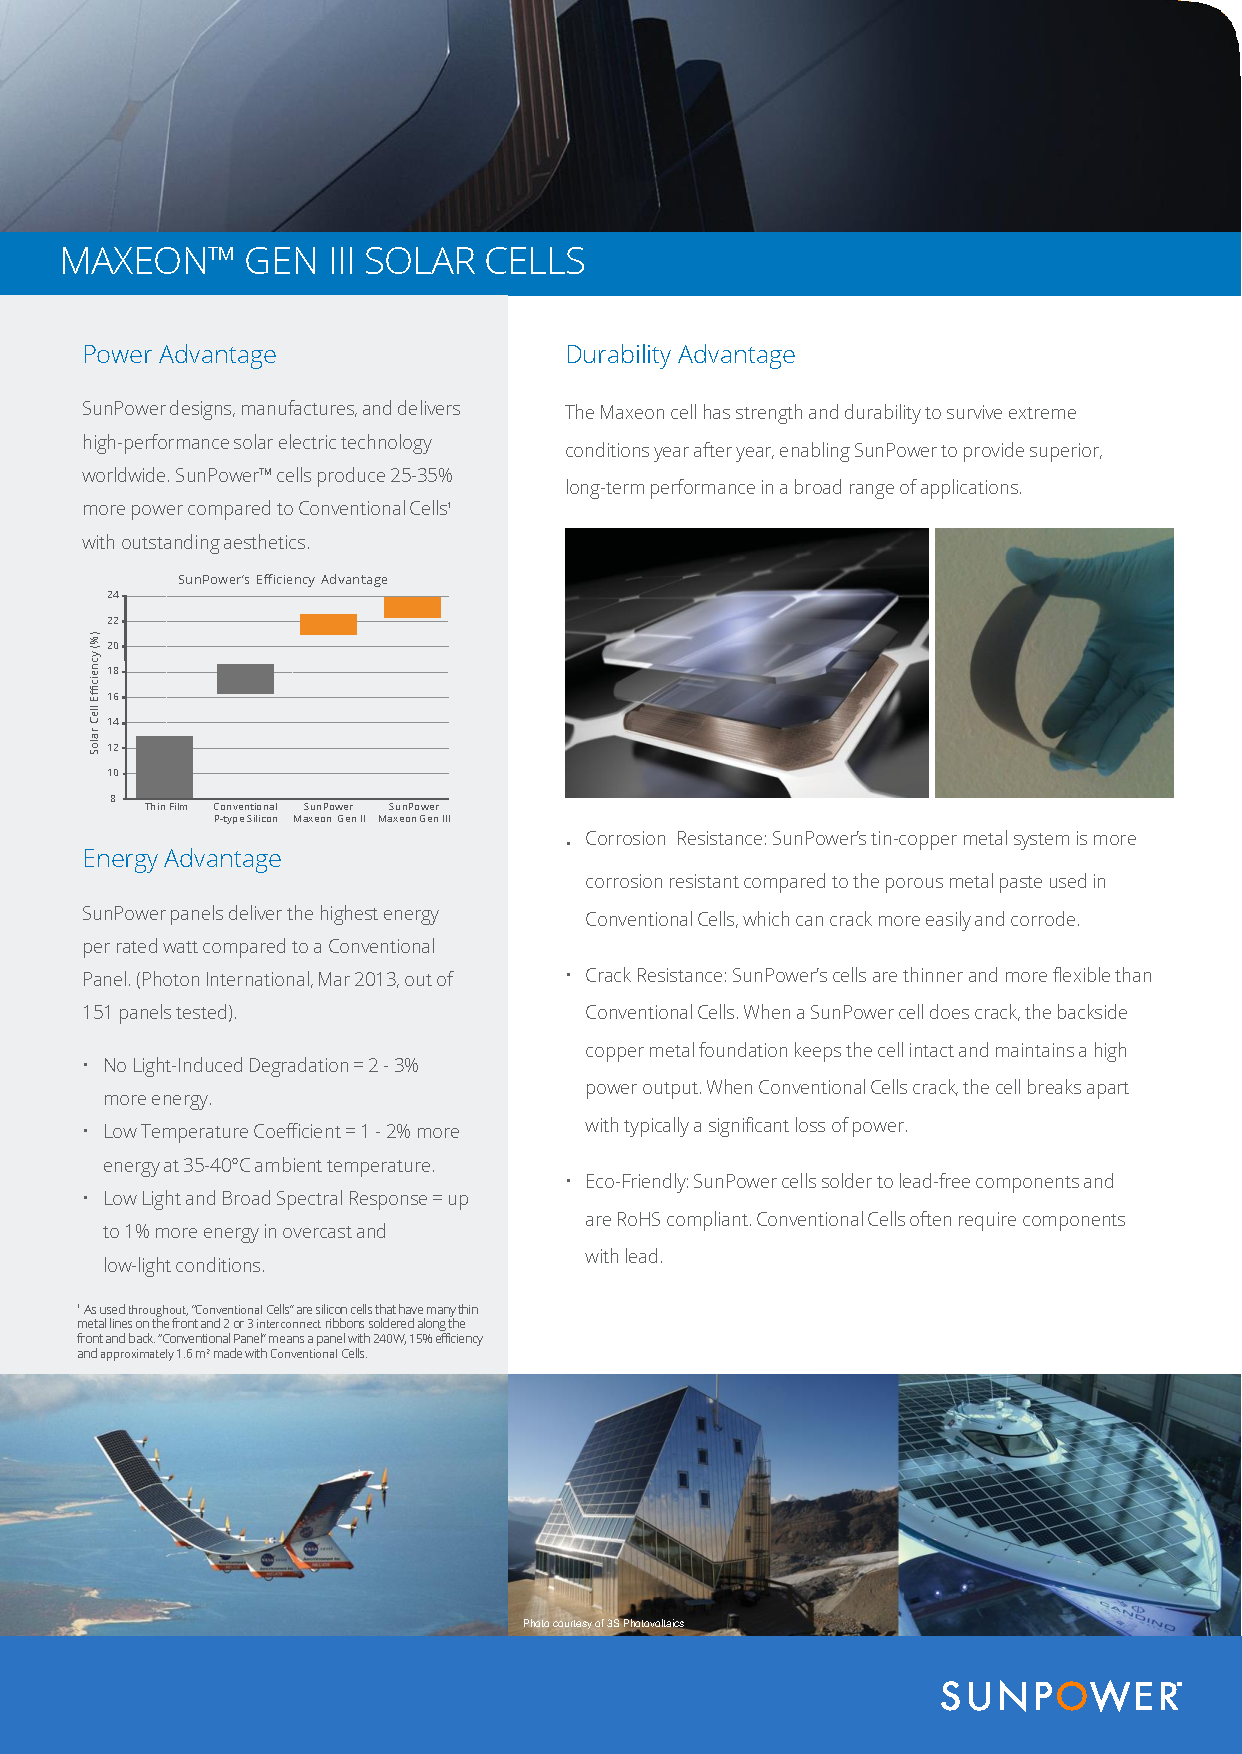
\includepdf[pages={-}]{pages/sunpower-maxeon-gen3.pdf}
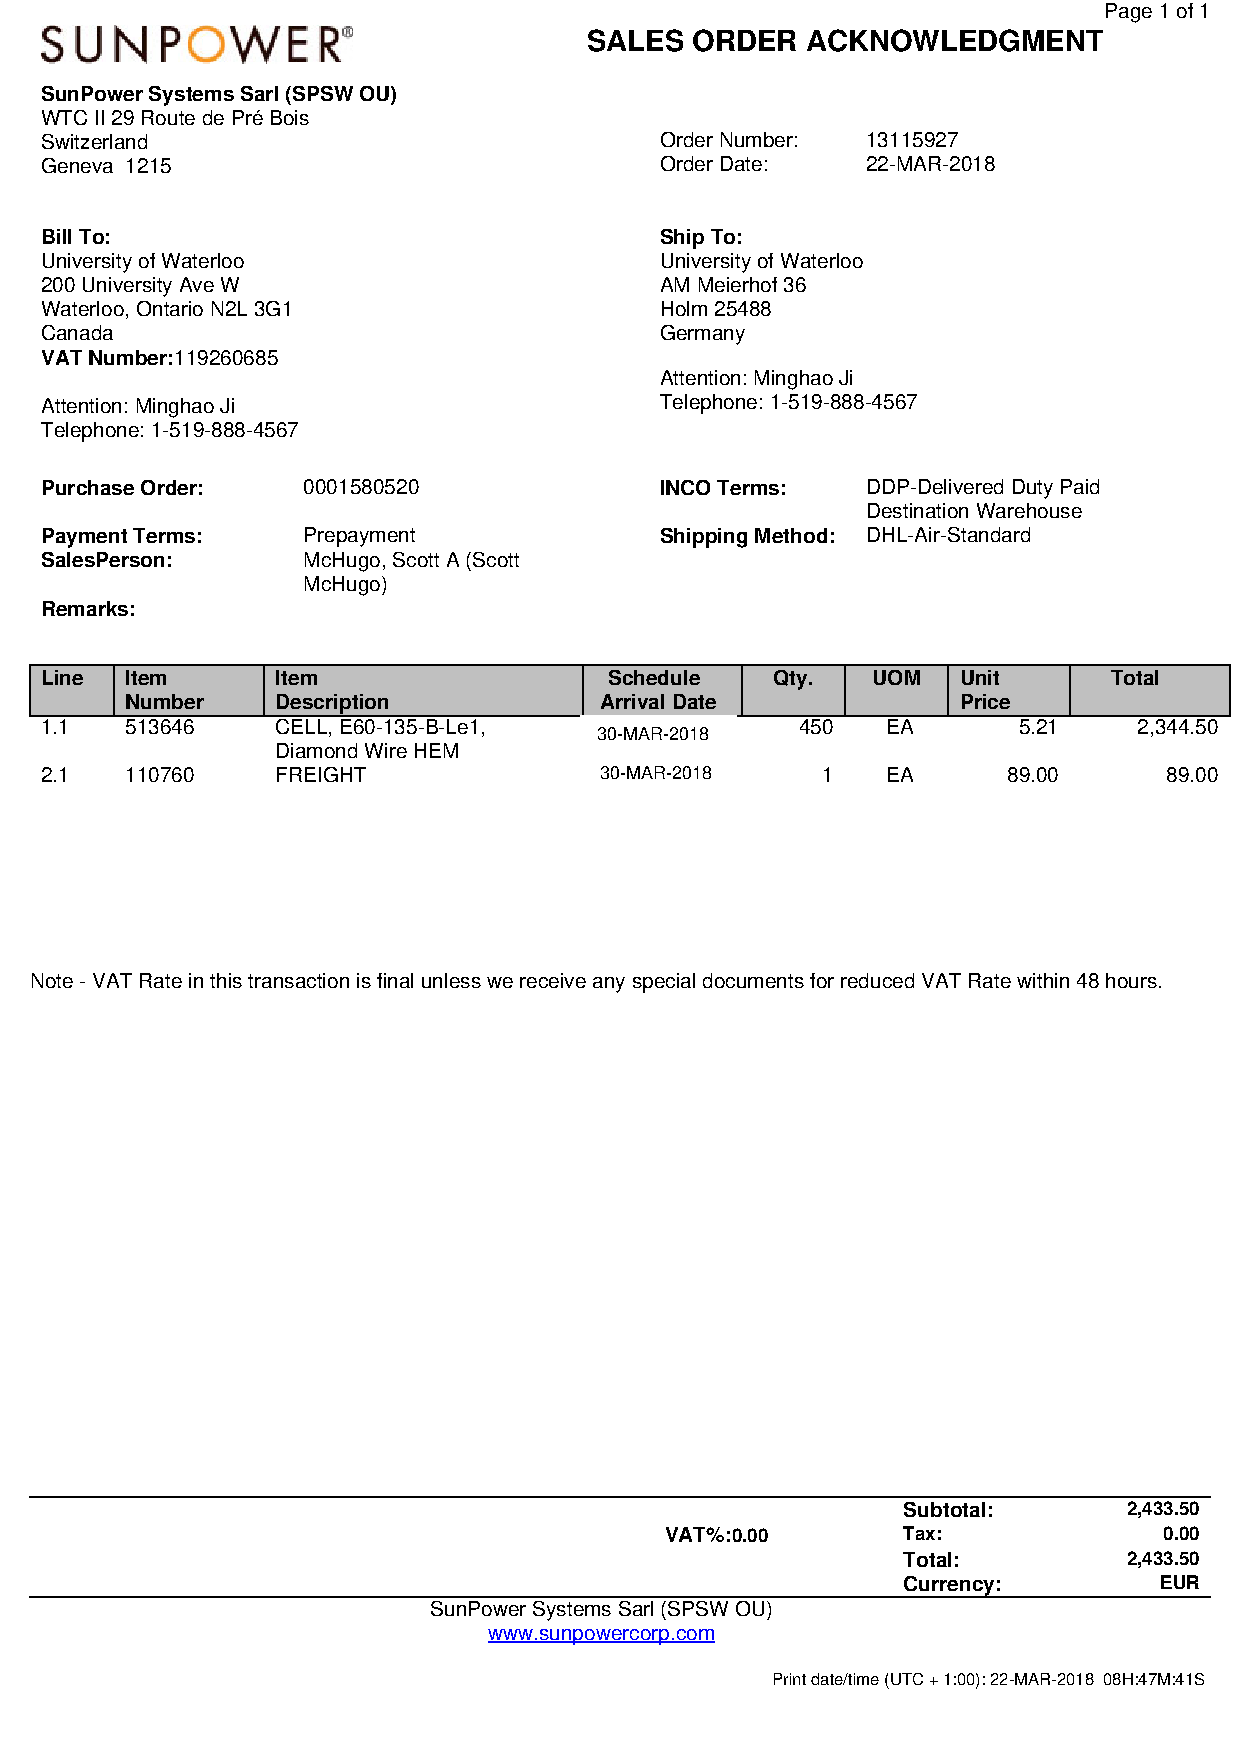
\includepdf[pages={-}]{pages/SOA_13115927.pdf}
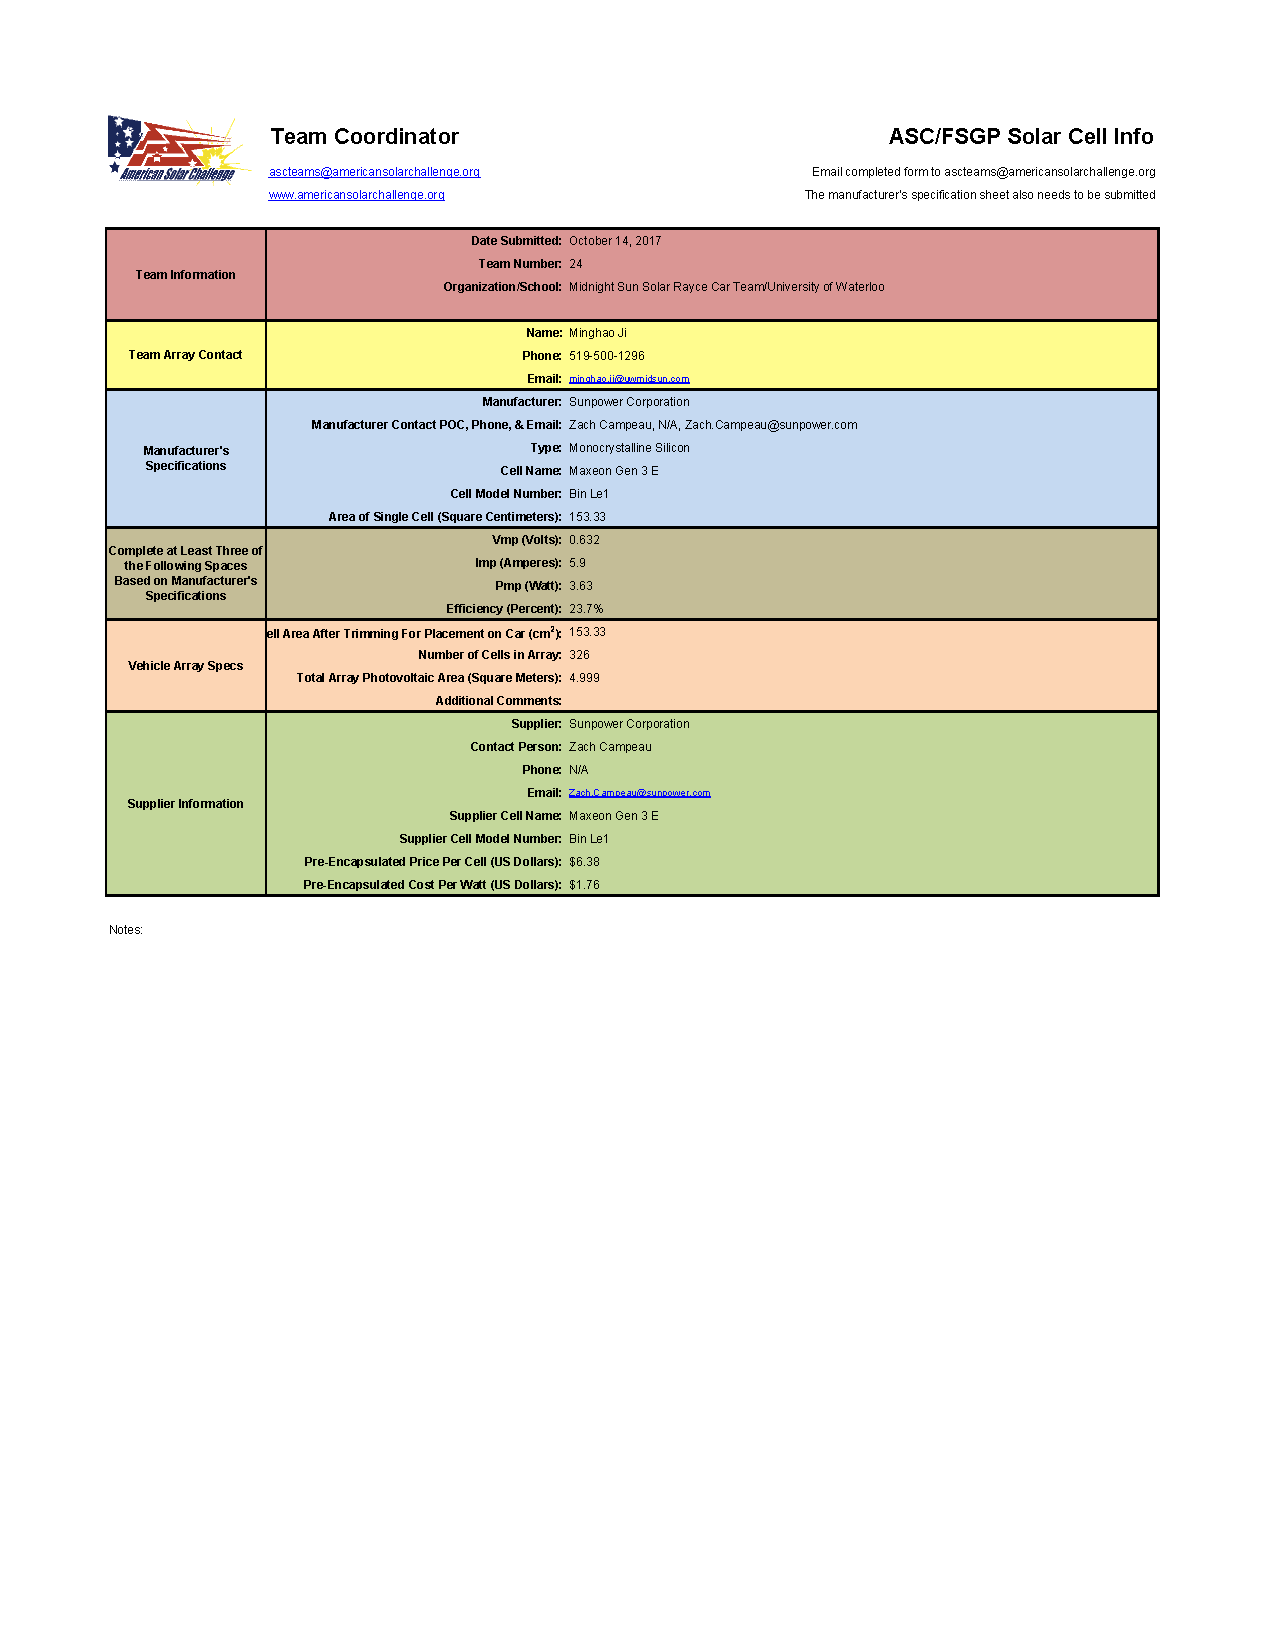
\includepdf[pages={-}]{pages/solar_cell_approval_form.pdf}

% Bibliography
%\pagebreak
%\printbibliography

% Appendix
\pagebreak
\appendix

\end{document}
